\documentclass[aspectratio=169,14pt]{beamer}

\usepackage{fontspec}
\usepackage{graphicx}
\usepackage{xcolor}
\usepackage{array}

\setsansfont[
  Path=final_assets/fonts/,
  UprightFont=AlegreyaSans-Light.ttf,
  ItalicFont=AlegreyaSans-LightItalic.ttf
]{AlegreyaSans}
\renewcommand{\familydefault}{\sfdefault}
\usefonttheme{professionalfonts}
\setbeamertemplate{navigation symbols}{}
\setbeamertemplate{footline}{}
\setbeamertemplate{headline}{}
\setlength{\parindent}{0pt}

\definecolor{Bg}{HTML}{F0F2F5}
\definecolor{Text}{HTML}{1E2A38}
\definecolor{Dim}{HTML}{4A5568}
\definecolor{Label}{HTML}{8896A7}
\definecolor{Rule}{HTML}{CDD2D9}
\definecolor{Surface}{HTML}{E6E9EE}

\setbeamercolor{background canvas}{bg=Bg}
\setbeamercolor{normal text}{fg=Text,bg=Bg}

\newcommand{\decklabel}[1]{%
  {\fontsize{8.5}{11}\selectfont\color{Label}\MakeUppercase{#1}\par}%
}
\newcommand{\slidetitle}[1]{%
  {\fontsize{25}{30}\selectfont\color{Text}\raggedright #1\par}%
}
\newcommand{\slidebody}[1]{%
  {\fontsize{12.2}{15.4}\selectfont\color{Dim}\raggedright #1\par}%
}
\newcommand{\smallbody}[1]{%
  {\fontsize{9.5}{12}\selectfont\color{Dim}\raggedright #1\par}%
}
\newcommand{\steplabel}[1]{%
  {\fontsize{9}{11}\selectfont\color{Text}#1\par}%
}
\newcommand{\stepbody}[1]{%
  {\fontsize{9.5}{12.0}\selectfont\color{Dim}\raggedright #1\par}%
}
\newcommand{\tinynote}[1]{%
  {\fontsize{8.5}{10}\selectfont\color{Label}#1\par}%
}
\newcommand{\thinrule}{%
  \par\vspace{0.24cm}%
  {\color{Rule}\rule{2.45cm}{0.35pt}}%
  \par\vspace{0.25cm}%
}

\begin{document}

% Voiceover target: 0:00--0:10
\begin{frame}[plain]
  \vspace*{0.72cm}
  \hspace*{1.22cm}
  \begin{minipage}{0.82\paperwidth}
    \raggedright
    \decklabel{CS 184 \textperiodcentered{} Spring 2026 \textperiodcentered{} Final Video}
    \vspace{0.62cm}

    {\fontsize{37}{44}\selectfont\color{Text}Limitless: Infinity\par}
    \vspace{0.25cm}
    {\fontsize{15.6}{20}\selectfont\color{Dim}Repulsive-surface optimization for self-intersection-free meshes.\par}
    \vspace{0.46cm}
    \textcolor{Rule}{\rule{2.45cm}{0.35pt}}
    \vspace{0.26cm}

    {\fontsize{9.5}{12}\selectfont\color{Label}
    Atharv Sampath \quad \textperiodcentered{} \quad Michael Pham
    \quad \textperiodcentered{} \quad Daniel Liu
    \quad \textperiodcentered{} \quad Elen Papyan\par}
  \end{minipage}
\end{frame}

% Voiceover target: 0:10--0:30
\begin{frame}[plain]
  \vspace*{0.82cm}
  \hspace*{1.22cm}
  \begin{minipage}{0.78\paperwidth}
  \raggedright
  \decklabel{01 -- The goal}
  \vspace{0.54cm}
  \slidetitle{Blend 3D shapes without them passing through themselves.}
  \thinrule
  \slidebody{Rather than detect collisions and resolve them, we encode repulsion in the energy itself. The energy is finite for any embedded surface and infinite the moment two patches meet, so starting from an embedded surface the optimizer cannot cross into a self-intersection.}
  \vspace{0.30cm}
  \slidebody{We descoped GPU acceleration after the milestone; everything in this video runs on CPU.}
  \end{minipage}
\end{frame}

% Voiceover target: 0:30--0:48
\begin{frame}[plain]
  \vspace*{0.82cm}
  \hspace*{1.22cm}
  \begin{minipage}{0.78\paperwidth}
  \raggedright
  \decklabel{02 -- The energy}
  \vspace{0.54cm}
  \slidetitle{Infinite at self-contact.}
  \thinrule
  \slidebody{The discrete tangent-point energy sums a kernel over triangle pairs. As two patches approach zero separation, the denominator vanishes and the kernel diverges.}
  \vspace{0.45cm}
  \begin{center}
  {\fontsize{12}{14}\selectfont\color{Text}
  $\displaystyle
    \widehat{\Phi}(x)
      = \sum_{t_1 \ne t_2}
        a_1 a_2 \,
        \frac{\bigl|\langle n_1,\, c_1 - c_2\rangle\bigr|^{6}}
             {\|c_1 - c_2\|^{12}}
  $%
  }
  \end{center}
  \end{minipage}
\end{frame}

% Voiceover target: 0:48--1:10
\begin{frame}[plain]
  \vspace*{0.45cm}
  \hspace*{1.22cm}
  \begin{minipage}{0.82\paperwidth}
  \raggedright
  \decklabel{03 -- The pipeline}
  \vspace{0.10cm}
  \slidetitle{Four steps, run every iteration.}
  \vspace{0.14cm}

  \renewcommand{\arraystretch}{1.05}
  \setlength{\tabcolsep}{4pt}
  \begin{tabular}{@{}p{2.9cm}p{9.7cm}@{}}
    \steplabel{1.\ Geometry} &
    \stepbody{Per-triangle centers, normals, and areas.} \\
    \steplabel{2.\ Fast energy} &
    \stepbody{Hierarchical clustering turns an O(n\textsuperscript{2}) sum into O(n log n).} \\
    \steplabel{3.\ Smooth descent} &
    \stepbody{A Sobolev-style preconditioner makes step size independent of mesh resolution.} \\
    \steplabel{4.\ Remeshing} &
    \stepbody{Edges split, collapse, and smooth so mesh quality stays controlled.} \\
  \end{tabular}
  \end{minipage}
\end{frame}

% Voiceover target: 1:10--1:35
\begin{frame}[plain]
  \vspace*{0.58cm}
  \hspace*{0.94cm}
  \begin{minipage}{0.84\paperwidth}
    \raggedright
    \decklabel{04 -- Canonical embeddings}
    \vspace{0.24cm}
    \slidetitle{Six surfaces flow toward embedded states.}
    \vspace{0.28cm}
    \begin{columns}[T,totalwidth=0.84\paperwidth]
      \begin{column}{0.49\paperwidth}
        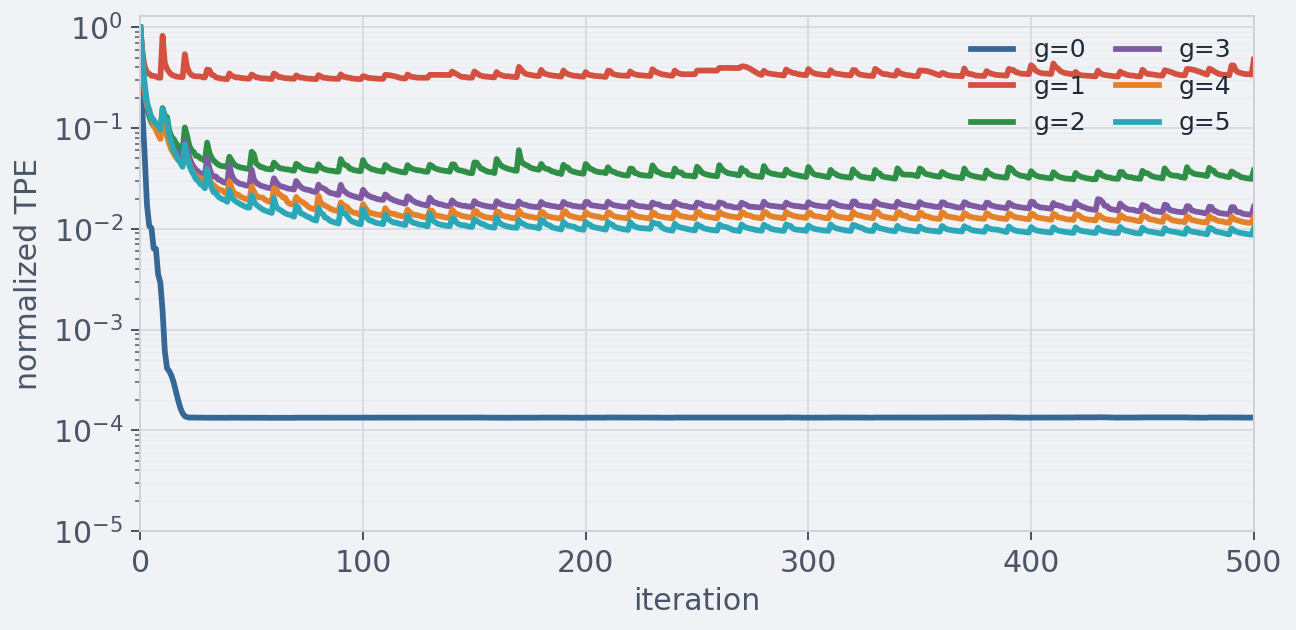
\includegraphics[width=\linewidth]{final_assets/gallery_energy_normalized.png}
      \end{column}
      \begin{column}{0.30\paperwidth}
        \smallbody{Tangent-point energy, normalized by the starting value, over 500 iterations on genus 0 through 5.}
        \vspace{0.22cm}
        \smallbody{Genus 0 collapses fastest because a sphere is the global minimum. Higher genera plateau into local minima with handles intact.}
        \vspace{0.22cm}
        \smallbody{Genus 1 is the stubborn case: starting near a torus of revolution leaves little energy to shed.}
      \end{column}
    \end{columns}
  \end{minipage}
\end{frame}

% Voiceover target: 1:35--2:00
\begin{frame}[plain]
  \vspace*{0.58cm}
  \hspace*{0.94cm}
  \begin{minipage}{0.84\paperwidth}
    \raggedright
    \decklabel{05 -- Sphere through a tube}
    \vspace{0.24cm}
    \slidetitle{A 30-frame collision-free path.}
    \vspace{0.28cm}
    \begin{columns}[T,totalwidth=0.84\paperwidth]
      \begin{column}{0.49\paperwidth}
        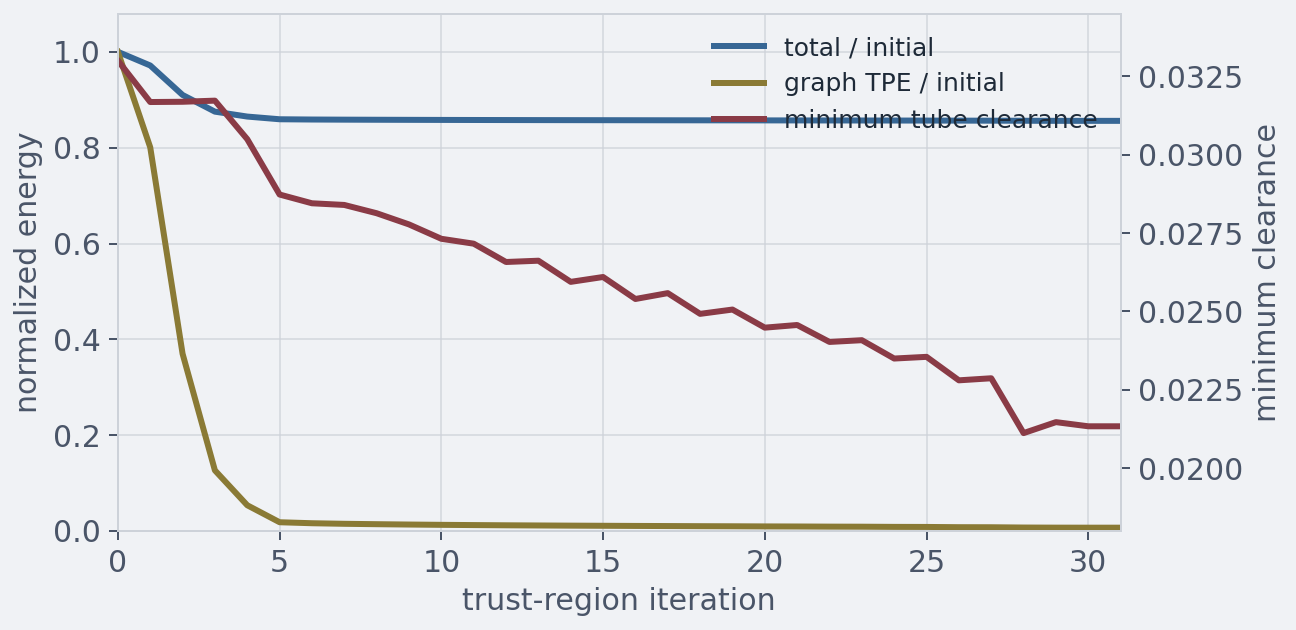
\includegraphics[width=\linewidth]{final_assets/ball_tube_energy.png}
      \end{column}
      \begin{column}{0.30\paperwidth}
        \smallbody{Trust-region descent on a path with fixed endpoints. The objective combines shell elasticity, self-repulsion, and a repulsive barrier from the tube surface.}
        \vspace{0.22cm}
        \smallbody{The path's self-repulsion term drops by two orders of magnitude in the first five iterations.}
        \vspace{0.22cm}
        \smallbody{The sphere stays clear of the tube wall for the full sequence.}
      \end{column}
    \end{columns}
  \end{minipage}
\end{frame}

% Voiceover target: 2:00--2:15
\begin{frame}[plain]
  \vspace*{0.82cm}
  \hspace*{1.22cm}
  \begin{minipage}{0.78\paperwidth}
  \raggedright
  \decklabel{06 -- Takeaway}
  \vspace{0.54cm}
  \slidetitle{A working repulsive-surface optimizer.}
  \thinrule
  \slidebody{We built the CPU core the full Repulsive Shells system depends on: fast tangent-point energy, preconditioned descent, dynamic remeshing, and a cross-validation harness against an external reference implementation.}
  \vspace{0.30cm}
  \slidebody{On top of that core, the graph-manifold path solver produced a collision-free sphere-through-tube interpolation. The pipeline is reproducible end-to-end from a saved frame sequence.}
  \end{minipage}
\end{frame}

\end{document}
